% Created 2022-02-02 Wed 14:55
% Intended LaTeX compiler: xelatex
\documentclass[11pt,twoside,twocolumn,landscape]{article}
\usepackage{graphicx}
\usepackage{longtable}
\usepackage{wrapfig}
\usepackage{rotating}
\usepackage[normalem]{ulem}
\usepackage{amsmath}
\usepackage{amssymb}
\usepackage{capt-of}
\usepackage{hyperref}
\usepackage[newfloat]{minted}
\usepackage{color}
\usepackage{listings}
\usepackage[top=2cm,bottom=2cm,right=2cm,left=2cm,landscape]{geometry}
\usepackage{multicol}
\usepackage{enumitem}
\usepackage{fancyhdr}
\usepackage{caption}
\usepackage{algorithm}
\usepackage{algpseudocode}
\setlist{noitemsep}
\setlength{\parindent}{0pt}
\setlength{\columnseprule}{0.2pt}
\definecolor{mygreen}{rgb}{0,0.6,0}
\definecolor{mygray}{rgb}{0.5,0.5,0.5}
\definecolor{mymauve}{rgb}{0.58,0,0.82}
\lstset{ backgroundcolor=\color{white}, basicstyle=\footnotesize, breaklines=true, captionpos=b, commentstyle=\color{mygreen}, escapeinside={\%*}{*)},keywordstyle=\color{blue}, stringstyle=\color{mymauve},}
\author{Olivier Lischer}
\date{\today}
\title{AlgDat Summary}
\hypersetup{
 pdfauthor={Olivier Lischer},
 pdftitle={AlgDat Summary},
 pdfkeywords={},
 pdfsubject={},
 pdfcreator={Emacs 27.2 (Org mode 9.5.1)}, 
 pdflang={English}}
\begin{document}

\pagestyle{fancy}
\fancyhf{}
\fancyhead[R]{AlgDat-HS21}
\fancyhead[L]{Exam Summary}
\fancyfoot[CE,CO]{\leftmark}
\fancyfoot[R]{\thepage}
\fancyfoot[L]{Olivier Lischer}

\tableofcontents
\newpage


\section{Data Structures}
\label{sec:orgca462ea}
\subparagraph{Binary Search Tree} \
\label{sec:orgbdbbcd1}
\begin{quote}
A Binary Search Tree is \href{../../../roam/20210806225200-binary_tree.org}{Binary Tree} which stores keys or key-value pairs so
that when you travel in-order all keys are sorted ascending.
\end{quote}

\subparagraph{AVLTree} \
\label{sec:orge9f4417}
An AVLTree is a special kind of \href{../../../roam/20211008140953-binary_search_tree.org}{Binary Search Tree}.
The AVLTree is self balancing and has therefore better running time guaranties than the normal \href{../../../roam/20211008140953-binary_search_tree.org}{Binary Search Tree}.
The tree rebalance itself when the \(abs(balance factor) > 1\).
The balance factor is calculated with: \texttt{BalanceFactor(Node) = Height(Node.LeftSubtree) - Height(Node.RightSubtree)}


For rebalancing exists two methods:
\begin{itemize}
\item \href{../../../roam/20211008144714-cut_link_algorithm.org}{Cut/Link Algorithm} aka. \href{../../../roam/20211008144714-cut_link_algorithm.org}{Trinode restructuring}
\item \href{../../../roam/20211008145521-rotation_balancing.org}{Rotation Balancing}
\end{itemize}

\emph{Running time}:
\begin{itemize}
\item find: \(O(\log (n))\)
\item insert: \(O(\log (n))\)
\begin{itemize}
\item at first find, after that restructure \(O(1)\)
\end{itemize}
\item delete: \(O(\log (n))\)
\begin{itemize}
\item at first find, after that restructure \(O(\log (n))\)
\end{itemize}
\end{itemize}

\subparagraph{Cut/Link Algorithm} \
\label{sec:org000babb}
This algorithm is used by some \href{../../../roam/20211008140953-binary_search_tree.org}{Binary Search Tree} for rebalancing. 

\begin{description}
\item[{Input}] A position \(x\) of a binary search tree \(T\) that has both a parent \(y\) and a grandparent \(z\)
\item[{Output}] Tree \(t\) after a trinode restructuring.
\end{description}


\begin{enumerate}
\item Let \((a, b, c)\) be a left-to-right (inorder) listing of the positions \(x\), \(y\) and \(z\), and let \((T_1, T_2, T_3, T_4)\) be a left-to-right (inorder) listing of the four subtrees of \(x\), \(y\) and \(z\) not rooted at \(x\), \(y\) and \(z\).
\item Replace the subtree rooted at \(z\) with a new subtree rooted at \(b\)
\begin{enumerate}
\item Let \(a\) be the left child of \(b\) and let \(T_1\) and \(T_2\) be the left and right subtrees of \(a\).
\item Let \(c\) be the right child of \(b\) and let \(T_3\) and \(T_4\) be the left and right subtrees of \(c\).
\end{enumerate}
\end{enumerate}




\begin{figure}[htbp]
\centering
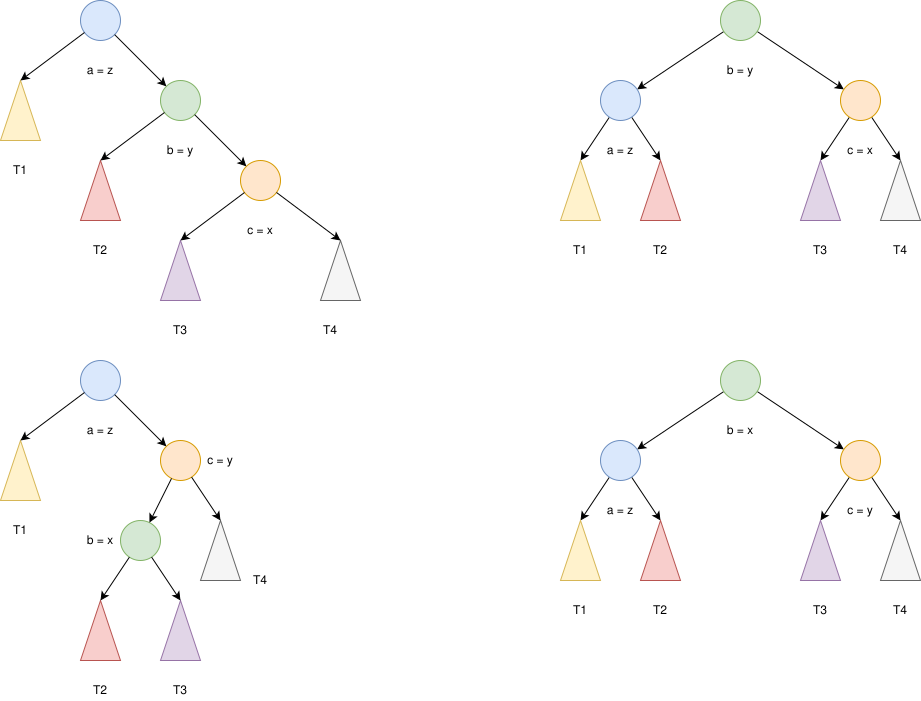
\includegraphics[width=.9\linewidth]{img/cut_link.drawio.png}
\caption{\label{fig:org8042c1d}Cut/Link Example}
\end{figure}

\subparagraph{Rotation Balancing} \
\label{sec:org85a8a5c}

This algorithm is used by some \href{../../../roam/20211008140953-binary_search_tree.org}{Binary Search Tree}s to restructure itself.
The problem with this technique is that you have to check what is required, a left rotation or a right rotation.
Some times a double rotation is required. 


\begin{description}
\item[{Input}] A position \(x\) of a binary search tree \(T\) that has both a parent \(y\) and a grandparent \(z\)
\item[{Output}] Tree \(t\) after a trinode restructuring.
\end{description}


\begin{enumerate}
\item Let \((a, b, c)\) the inorder listing of the positions \(x\), \(y\), \(z\)
\item Do the required rotations until \(b\) is at the top.
\end{enumerate}


\lstset{language=java,label= ,caption= ,captionpos=b,numbers=none}
\begin{lstlisting}
// right rotation
BinaryNode rotateWithLeftChild(BinaryNode k2) {
    BinaryNode k1 = k2.left;
    k2.left = k1.right;
    k1.right = k2;
    return k1;
}

// left rotation
BinaryNode rotateWithRightChild( BinaryNode k1 ) {
    BinaryNode k2 = k1.right; // Hilfsknoten
    k1.right = k2.left;
    k2.left = k1;
    return k2;
}
\end{lstlisting}



\subparagraph{Splay Tree} \
\label{sec:org04358b4}

A Splay Tree is a \href{../../../roam/20211008140953-binary_search_tree.org}{Binary Search Tree} which moves the accessed note after the operation to the root.
Even after update or search.
Moving the accessd note to the root is achived using rotation.
You rotate until the access element is at the top.
Splay Trees are usefull when you search often for the same thing.

\begin{figure}[htbp]
\centering
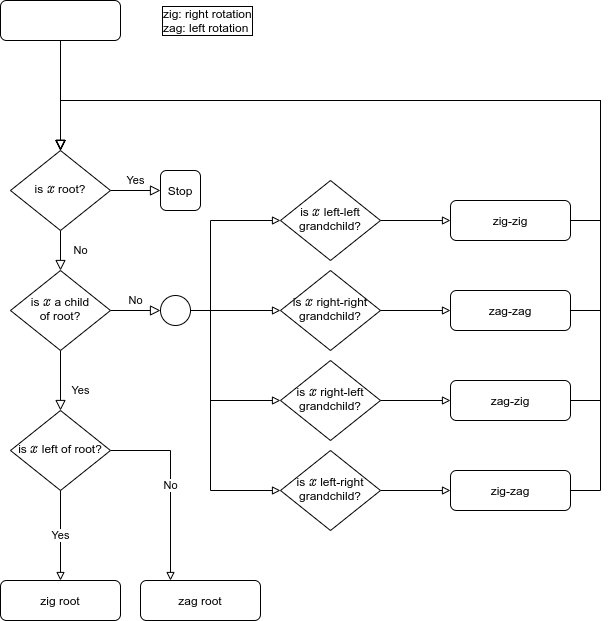
\includegraphics[width=.9\linewidth]{img/splaying.png}
\caption{\label{fig:orgf3295e2}Splaying Algorithm}
\end{figure}

\subparagraph{Graph} \
\label{sec:orgf5931d5}

A graph consist of \textbf{Vertices} and \textbf{Edges}.
It exists directed and undirected edges / graphs.
A directed edge has one start node and one end node.
An undirected edge has two nodes which are whether start nor end node.
In a directed graph (Digraph) all edges are directed.
In an undirected graph all edges are undirected.


A Graph is called connected when between every pair of vertices a path exists.

\subparagraph{Graph Terminology} \
\label{sec:org0269bc4}

The Terminology used when working with graphs (\href{../../../roam/20220201163000-graph.org}{Graph}).


\begin{itemize}
\item Edges are \textbf{incident} (finished) on a vertex
\begin{itemize}
\item \(a, d, b\) are incident in \(V\)
\end{itemize}
\item \textbf{Adjacent} (neighboring) vertices
\begin{itemize}
\item \(U, V\) are adjacent
\end{itemize}
\item \textbf{Degree} of a Vertex: The number of incident edges
\begin{itemize}
\item \(X\) has degree 5
\end{itemize}
\item \textbf{Parallel edges}
\begin{itemize}
\item \(h, i\) are parallel
\end{itemize}
\item \textbf{Loop}
\begin{itemize}
\item \(j\) is a loop
\end{itemize}
\item \textbf{Path}
\begin{itemize}
\item Sequence of vertices and edges
\item starts with a vertex and ends with a vertex
\end{itemize}
\item \textbf{Simple Path}
\begin{itemize}
\item all vertices and edges are unique
\end{itemize}
\item \textbf{Cycle}
\begin{itemize}
\item cyclic sequence of vertices and edges
\end{itemize}
\item \textbf{Simple Cycle}
\begin{itemize}
\item all vertices and edges are unique
\end{itemize}
\item \textbf{Strong Connectivity}
\begin{itemize}
\item every vertex can reach every other vertex
\end{itemize}
\item \textbf{Distance}
\begin{itemize}
\item The distance of a vertex \(v\) to a vertex \(w\) is the length of the shortest path between \(v\) and \(w\)
\end{itemize}
\end{itemize}


\begin{figure}[htbp]
\centering
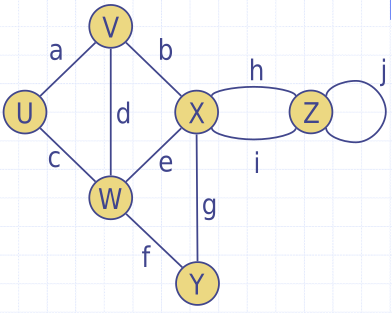
\includegraphics[width=.9\linewidth]{img/graph_example.png}
\caption{\label{fig:orga771366}Graph Example}
\end{figure}

\subparagraph{How to Store a graph} \
\label{sec:org4c4fd20}

To store a graph you have a few possibilities.
\begin{itemize}
\item \href{../../../roam/20220201173524-edge_list_structure.org}{Edge List Structure}
\item \href{../../../roam/20220201180442-adjacent_list_structure.org}{Adjacent List Structure}
\item \href{../../../roam/20220201180955-adjacent_matrix_structure.org}{Adjacent Matrix Structure}
\end{itemize}


\begin{figure}[htbp]
\centering
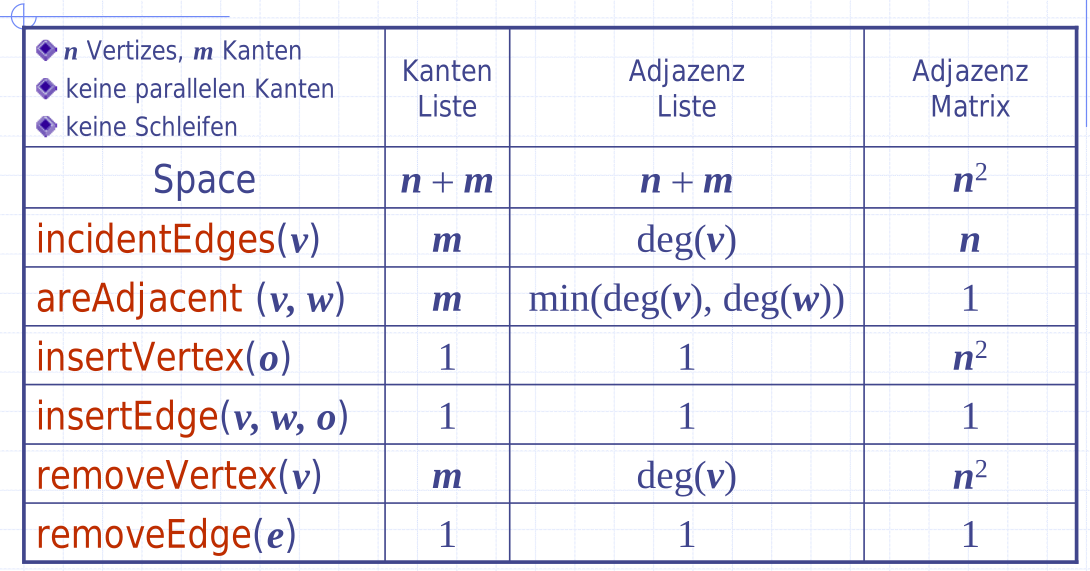
\includegraphics[width=.9\linewidth]{img/graph_data_structure_summary_running_time.png}
\caption{\label{fig:org8ab9949}Performance Summary for Graph Data Structures}
\end{figure}

\subparagraph{Edge List Structure} \
\label{sec:org4e20781}

To represent a \href{../../../roam/20220201163000-graph.org}{Graph} you could use the Edge list Structure.

The Edge List Structure stores the nodes in a list.
The Edge objects are also stored in a list.
Each edge object holds a reference to the start vertex and to the end reference.


\begin{figure}[htbp]
\centering
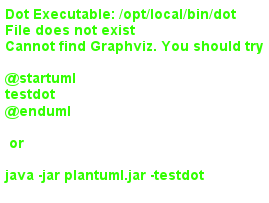
\includegraphics[width=.9\linewidth]{img/edge_list_structure.png}
\caption{Test}
\end{figure}


\subparagraph{Adjacent list Structure} \
\label{sec:org6b2a59e}

To represent a \href{../../../roam/20220201163000-graph.org}{Graph} you could use the Adjacent list Structure.

The Adjacent List Structure stores the nodes in a list.
The Edge objects are also stored in a list.
Each edge object holds a reference to the start vertex and to the end reference.
The Vertex object holds a list with references to the edge objects.


\begin{center}
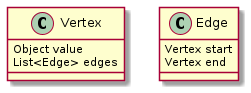
\includegraphics[width=.9\linewidth]{img/adjacent_list_structure.png}
\end{center}

\subparagraph{Adjacent Matrix Structure} \
\label{sec:org00d0e65}

To represent a \href{../../../roam/20220201163000-graph.org}{Graph} you could use the Adjacent Matrix Structure.

The Adjacent Matrix Structure stores the nodes in a list.
The Edge objects are also stored in a list.
Each edge object holds a reference to the start vertex and to the end reference.
Additionally you have a \(n \times n\) matrix / array.
The indexes represent vertexies in the vertex list.
If a edge exists between node 0 and node 1 then in \(M[0][1]\) a edge object is stored.
If no connection exists the null value is there. 



\begin{center}
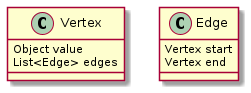
\includegraphics[width=.9\linewidth]{img/adjacent_matrix_structure.png}
\end{center}

\subparagraph{Subgraph} \
\label{sec:org94c047c}

A \textbf{Subgraph} \(S\) of \(G\) is \href{../../../roam/20220201163000-graph.org}{Graph} which contains a set subset of vertices and edges of the Graph \(G\).
A \textbf{Spanning Subtree} \(S\) of \(G\) is a graph which contains all vertices of the graph \(G\)

\subparagraph{Special Kind of Graph / Trees} \
\label{sec:org023ff15}

A free tree \(T\) is a undirected graph (\href{../../../roam/20220201163000-graph.org}{Graph}) so that T is conected an has no cycles.
A forest is a graph without cycles
A Spanning Tree of a connected graph is a \href{../../../roam/20220201181419-subgraph.org}{Subgraph} which is also tree

\subparagraph{Transitory Clousre} \
\label{sec:org3720884}

The Transitory closure of a Digraph (\href{../../../roam/20220201163000-graph.org}{Graph}) \(G\) is another Digraph \(G*\) which:
\begin{itemize}
\item has the same vertices as \(G\)
\item when in \(G\) a directed path betwenn \(u\) and \(v\) exists (\(u \ne v\)) then has \(G*\) a directed edge from \(u\) to \(v\)
\end{itemize}

To calculate the Transitory Closure the \href{../../../roam/20220202113404-the_floyd_warshall_algorithm.org}{The Floyd-Warshall Algorithm} is used.


\begin{figure}[htbp]
\centering
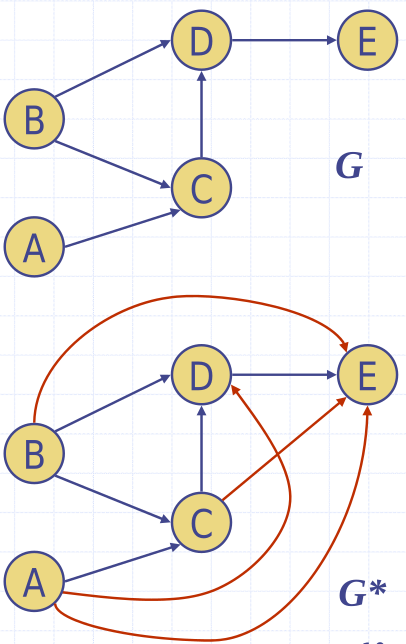
\includegraphics[width=.9\linewidth]{img/transitiver_abschluss.png}
\caption{\label{fig:orge58c570}Transitory Clousre}
\end{figure}

\subparagraph{DAG} \
\label{sec:org09da1c6}

A DAG is directed acyclic graph.
A \href{../../../roam/20220201163000-graph.org}{Graph} without directed cycles.


\begin{figure}[htbp]
\centering
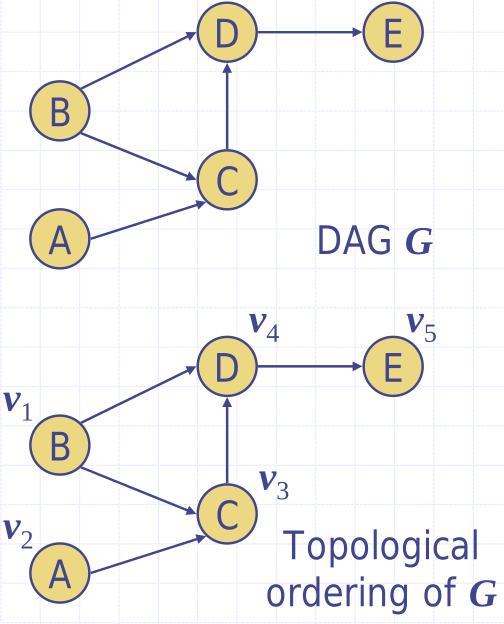
\includegraphics[width=.9\linewidth]{img/dag.png}
\caption{\label{fig:org45ff59c}DAG Example}
\end{figure}

\section{Algorithms}
\label{sec:org41f9e46}
\subparagraph{Merge Sort} \
\label{sec:orgbbe3c14}

\begin{description}
\item[{Running time}] \(O(n \log(n))\)
\end{description}

Merge Sort uses the Divide-and-Conquer principle.
It divides the list into 2 splits and the each list again into two lists until the list length is 1.
After that the two lists are merged.
The resulting lists are merged again until you have the sorted list.
\lstset{language=java,label= ,caption= ,captionpos=b,numbers=none}
\begin{lstlisting}
public static <T extends Comparable<? super T>> T[] mergeSort(T[] s) {  
  int n = s.length;
  if (n > 1) {
    T[] s1 = Arrays.copyOfRange(s, 0, n/2);
    T[] s2 = Arrays.copyOfRange(s, n/2, n);
    s1 = mergeSort(s1);
    s2 = mergeSort(s2);
    s = merge(s1, s2);
  }
  return s;
}

static <T extends Comparable<? super T>> T[] merge(T[] a, T[] b) {
  T[] s = newInstance(a, a.length * 2);
  int ai = 0; // First Element in 'Sequence' A
  int bi = 0; // First Element in 'Sequence' B
  int si = 0; // Last Element in 'Sequence' S
  while (!(ai == a.length) && !(bi == b.length)) {
    if (a[ai].compareTo(b[bi]) < 0) {
      s[si++] = a[ai++];
    }
    else {
      s[si++] = b[bi++];
    }
  }
  while (!(ai == a.length)) {
    s[si++] = a[ai++];
  }
  while (!(bi == b.length)) {
    s[si++] = b[bi++];
  }
  return s;
}
\end{lstlisting}

\begin{figure}[htbp]
\centering
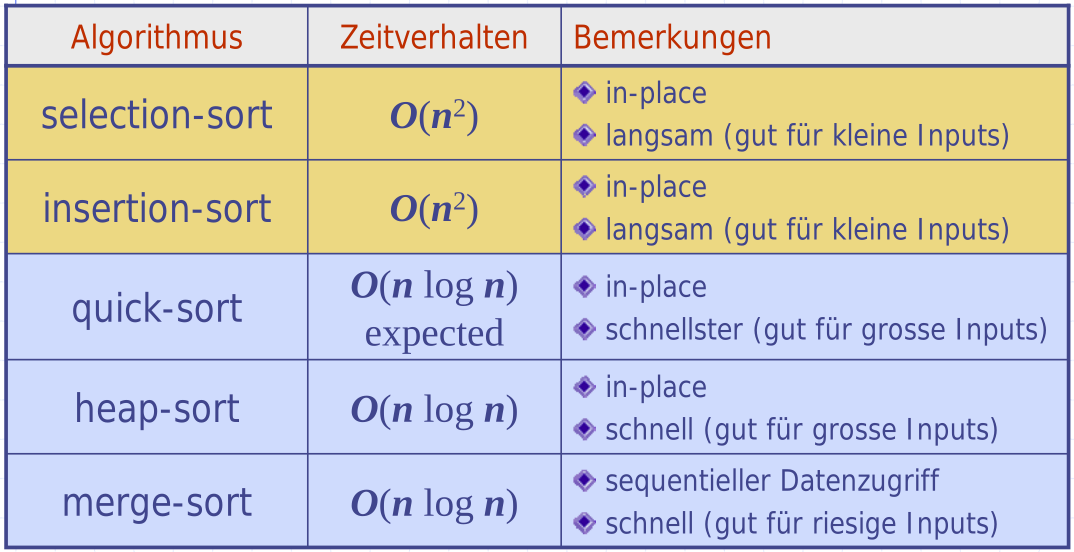
\includegraphics[width=.9\linewidth]{img/sort_algorithm_summary_runtime.png}
\caption{\label{fig:org4250f3e}Runtime Summary}
\end{figure}

\subparagraph{Quick Sort} \
\label{sec:org76821a9}

\begin{description}
\item[{running time}] \(O(n \log(n))\) expected
\end{description}

Quick Sort uses the Divide-and-Conquer principle.
\begin{enumerate}
\item A random element \(x\) is choosen (the \textbf{pivot}).
\item Divide
\begin{enumerate}
\item All elements smaller than \(x\) go to \(S\)
\item All elements greater than \(x\) go to \(G\)
\item All elements equal \(x\) go to \(E\)
\end{enumerate}
\item Repeate 2 for each list until list length 1
\item merge from lower to equal to higher
\end{enumerate}


\begin{figure}[htbp]
\centering
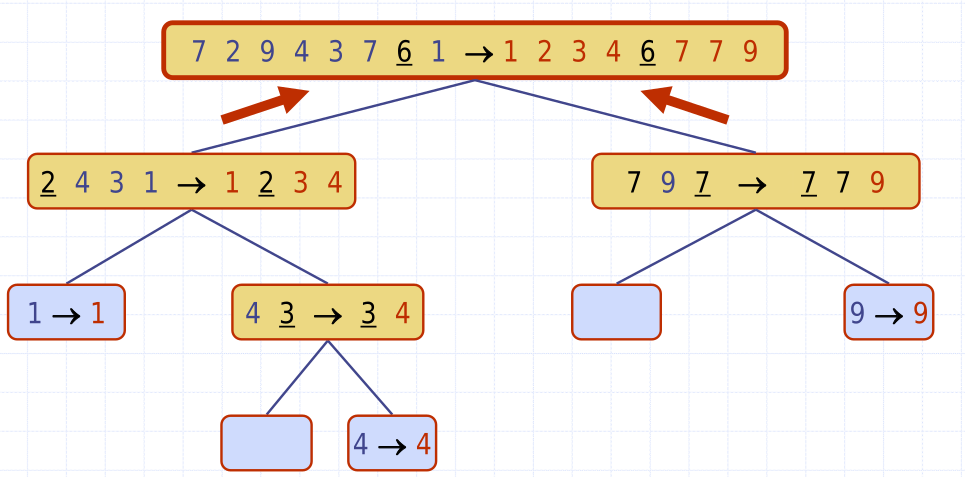
\includegraphics[width=.9\linewidth]{img/quick_sort_tree.png}
\caption{\label{fig:org6dea0f5}Quick Sort Tree}
\end{figure}

\lstset{language=java,label= ,caption= ,captionpos=b,numbers=none}
\begin{lstlisting}
/*
 * @param a
 *          The leftbound of the part that shall be sorted.
 * @param b
 *          The rightbound of the part that shall be sorted.
 */
public <T> void inPlaceQuickSort(T[] sequence, Comparator<T> comp, int a, int b) {
    T temp;
    if (a >= b)
	return;
    T pivot = sequence[b];
    int l = a;
    int r = b - 1;
    while (l <= r) {
	while (l <= r && comp.compare(sequence[l], pivot) <= 0) {
	    l++;
	}
	while (r >= l && comp.compare(sequence[r], pivot) >= 0) {
	    r--;
	}
	if (l < r) {
	    temp = sequence[l];
	    sequence[l] = sequence[r];
	    sequence[r] = temp;
	}
    }
    temp = sequence[l];
    sequence[l] = sequence[b];
    sequence[b] = temp;
    /*  Move index if sequence of equal elements. E.g.:
     *  |---+---+---+---+---+---+---+---+---+---+---+---+---|
     *  |   |   | 5 | 5 | 2 | 8 | 8 | 8 | 8 |   |   |   |   |
     *  |---+---+---+---+---+---+---+---+---+---+---+---+---|
     *    a                   l <-------- l               b
     */
    while ((l > a) && (comp.compare(sequence[l], sequence[l-1]) == 0)) { 
	l--;
    }
    while ((r < b) && (r > a) && (comp.compare(sequence[r], sequence[r+1]) == 0)) {
	r++;
    }
    inPlaceQuickSort(sequence, comp, a, l - 1);
    inPlaceQuickSort(sequence, comp, r + 1, b);
}
\end{lstlisting}

\subparagraph{Lower Bound Search Algorithm} \
\label{sec:orge02673d}

Every sorting algorithm which uses comparing has a minimal running time of \(\log(n!)\).
In O notation this is \(O(n \log(n))\).

\begin{align}
\log(n!) &\geq \log{(\frac{n}{2})^{\frac{n}{2}}} = \frac{n}{2}\log(\frac{n}{2}) \\
n! &\geq \sqrt{2\pi \cdot n}(\frac{n}{2})^2 \rightarrow O(n \log n)
\end{align}

\subparagraph{Bucket Sort} \
\label{sec:org1b5c314}

\begin{description}
\item[{running time}] \(O(n + N)\)
\end{description}

Bucket Sort is Sorting algorithm which does not use any compares to achieve the sorting.

To sort something with bucket sort you need a key.
This key must have a specific range \([0, N-1]\).
Then you create an array of \(N\) empty lists.
Then you move the value from initial unsorted list into the array.
The key of the element specifies the location in the array.
After the initial list is cleared you filled again by iterating over the array.

\lstset{language=java,label= ,caption= ,captionpos=b,numbers=none}
\begin{lstlisting}
public List<T> bucketSort(List<T> S, int N) {
    List<T>[] buckets = new ArrayList[N];

    while (!S.isEmpty()) {
	T f = S.first();
	(k,o) = S.remove(f);
	buckets[k].insertLast((k,o));
    }

    for (int i = 0; i < N; i++) {
	while (!buckets[i].isEmpty()) {
	    T f = buckets[i].first();
	    (k,o) = B[i].remove(f);
	    S.insertLast((k,o));
	}
    }
}

\end{lstlisting}

\subparagraph{Radix Sort} \
\label{sec:org2b2f972}

Radix Sort is a sorting algorithm for lexicographical sorting based on \href{../../../roam/20211215102604-bucket_sort.org}{Bucket Sort}.

\begin{figure}[htbp]
\centering
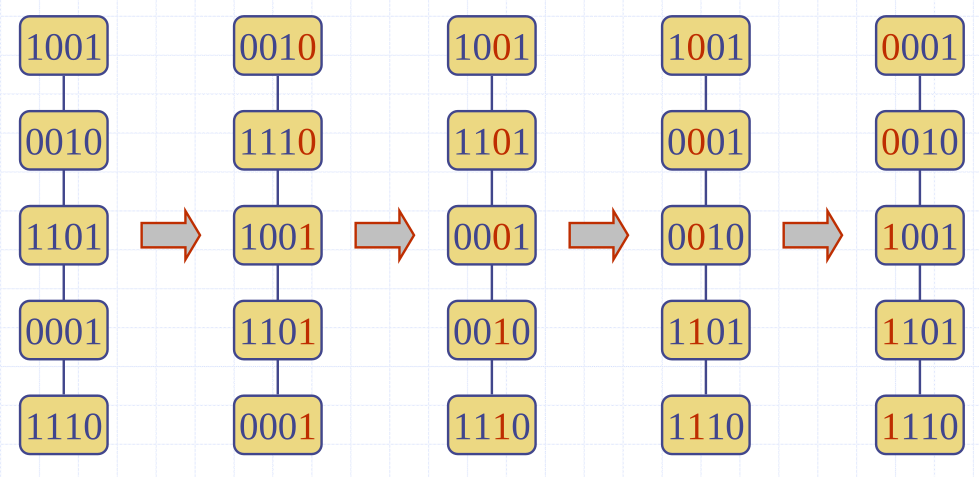
\includegraphics[width=.9\linewidth]{img/radix_sort.png}
\caption{\label{fig:org9e75117}Radix Sort of a 4-Bit Integer}
\end{figure}

\lstset{language=java,label= ,caption= ,captionpos=b,numbers=none}
\begin{lstlisting}
public void radixSort(String[] data) {
  // find max string-length
  int maxLength = -1;
  OptionalInt max = Arrays.stream(data).mapToInt(str -> str.length()).max();
  if (max.isPresent()) {
    maxLength = max.getAsInt();
  } else {
    return;
  }

  // bucketsort from max index to first index
  for (int i = maxLength - 1; i >= 0; i--) {
    bucketSort(data, i);
  }

}

protected void bucketSort(String[] data, int index) {
  Arrays.stream(data).forEachOrdered(str -> {
    if (str.length() <= index) {
      buckets[0].addLast(str);
    } else {
      buckets[str.charAt(index) - 'a' + 1].addLast(str);
    }
  });

  String[] phase2Array = Arrays.asList(buckets).stream().flatMap(List::stream)
      .toArray(String[]::new);
  System.arraycopy(phase2Array, 0, data, 0, phase2Array.length);
  Arrays.stream(buckets).parallel().forEach(list -> list.clear());
}
\end{lstlisting}

\subparagraph{Boyere-Moore} \
\label{sec:org25d64b0}

\begin{description}
\item[{running time}] \(O(n\cdot m + s)\)
\end{description}

The Boyere-Moore Algorithm is used for \href{../../../roam/20211215163350-pattern_matching.org}{Pattern Matching}.
Instead to compare the pattern from the beginning it starts at the end.

\begin{enumerate}
\item align start character of search string with pattern
\item compare the n-th character of pattern with search string
\item chars equal: \(n = n-1\) and go to 2.
\item not equal: move pattern forward
\begin{enumerate}
\item mismatched character occurs: move pattern forward to mismatched (last occurence function)
\item else: move whole pattern after the mismatched position
\end{enumerate}
\end{enumerate}


The last occurence funciton returns the index of the where the charachter \(x\) occurs last in the pattern (\ref{fig:orgca53813}).

\begin{figure}[htbp]
\centering
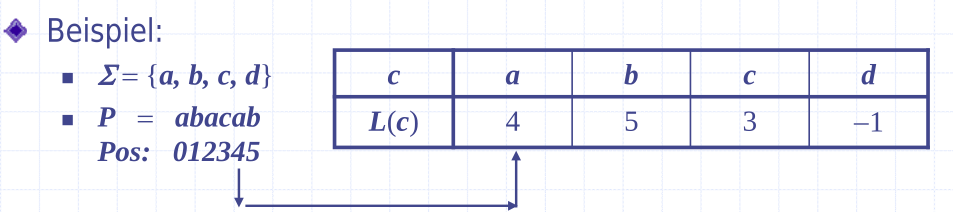
\includegraphics[width=.9\linewidth]{img/lastOccurrence.png}
\caption{\label{fig:orgca53813}Last Occurrence Function}
\end{figure}

\begin{figure}[htbp]
\centering
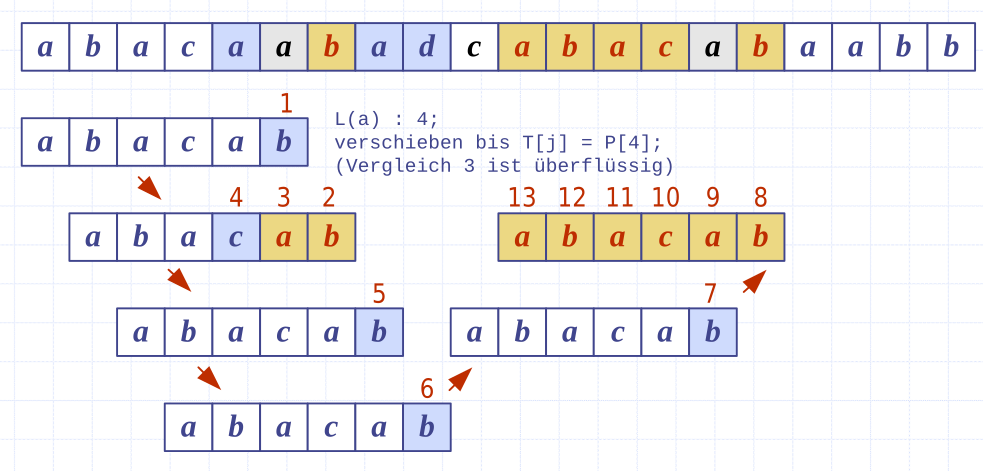
\includegraphics[width=.9\linewidth]{img/boyere_moore.png}
\caption{Boyere-Moore Algorithm}
\end{figure}


\begin{algorithm}
  \caption{Boyer-Moore Algorithm}
  \begin{algorithmic}[1]
    \Procedure{BoyerMooreMatch}{$T, P, \Sigma$}
    \State $L \leftarrow lastOccurenceFunction(P, \Sigma)$
    \State $i \leftarrow m - 1$
    \State $j \leftarrow m - 1$
    \Repeat
    \If{$T[i] = P[j]$}
    \If{$j = 0$}
    \State \textbf{return $i$} \{ match at i \}
    \Else
    \State $i \leftarrow i - 1$
    \State $j \leftarrow j - 1$
    \EndIf
    \State \{ charchter-jump \}
    \State $l \leftarrow L[T[i]]$
    \State $i \leftarrow i + m - min(j, 1 + l)$
    \State $j \leftarrow m - 1$
    \EndIf
    \Until{$i > n - 1$}
    \State \textbf{return} $b$ \{ The gcd is b \}
    \EndProcedure
  \end{algorithmic}
\end{algorithm}

\subparagraph{KMP} \
\label{sec:org57d450e}

\begin{description}
\item[{running time}] O(m + n)
\end{description}


The KMP Algorithm is a \href{../../../roam/20211215163350-pattern_matching.org}{Pattern Matching} Algorithm.
KMP compares the pattern with text from left to right.
But it moves the pattern smarter than Brute-Force.

The Algorithm has two phases:
\begin{enumerate}
\item calculating the \textbf{failure function}
\begin{itemize}
\item \href{../../../roam/20211215171140-calculating_the_failure_function_for_kmp.org}{Calculating the Failure Function for KMP}
\end{itemize}
\item the actual pattern matching
\end{enumerate}


\begin{enumerate}
\item If \(T[i] = P[i]\)
\begin{enumerate}
\item is pattern found, then return start position
\item otherwise increment \(i\) and \(j\)
\end{enumerate}
\item otherwise if \(j > 0\) 
\begin{enumerate}
\item then \(j\) will become the value from the \(failureFunction(j)\)
\item else \$i = i + \$
\end{enumerate}
\end{enumerate}


\textbf{Example:}

KMP according to figure \ref{fig:org00980dd}:
\begin{enumerate}
\item the first 5 comparisons are matching
\item 6 does not match
\begin{enumerate}
\item check if 5 could be an prefix (failure function)
\item yes, the first character of the pattern must not be compared
\end{enumerate}
\item 7 does not match
\begin{enumerate}
\item check error function
\item 0 \(\rightarrow\) align pattern to current position
\end{enumerate}
\item and so on
\end{enumerate}

\begin{figure}[htbp]
\centering
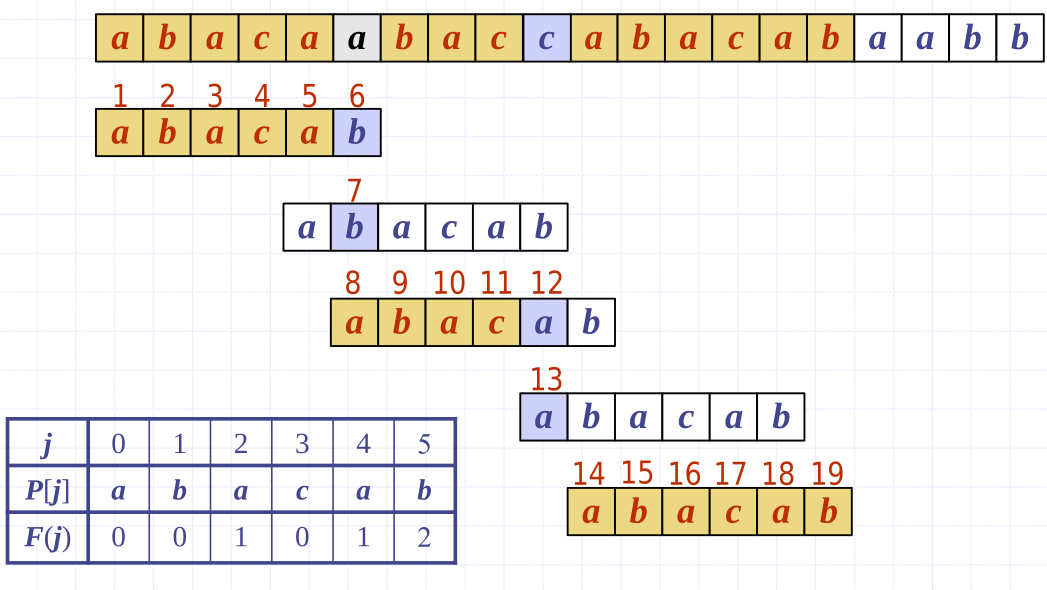
\includegraphics[width=.9\linewidth]{img/kmp_example.png}
\caption{\label{fig:org00980dd}KMP Example}
\end{figure}


\begin{algorithm}
  \caption{KMP Algorithm}
  \begin{algorithmic}[1]
    \Procedure{KMPMatch}{$T, P$}
    \State $F \leftarrow failureFunction(P)$
    \State $i \leftarrow 0$ \{ Location in search string \}
    \State $j \leftarrow 0$ \{ Location in pattern \}
    \While{$i < m-1$}
    \If{$T[i] = P[i]$}
    \If{$j = m - 1$} \{ m length of pattern \}
    \State \textbf{return} $i - m + 1$ \{ match \}
    \Else
    \State $i \leftarrow i + 1$
    \State $j \leftarrow j + 1$
    \EndIf
    \Else
    \If{$j > 0$}
    \State $j \leftarrow F[j-1]$
    \Else
    \State $i \leftarrow i + 1$
    \EndIf
    \EndIf
    \EndWhile
    \textbf{return} -1 \{ no match \}
    \EndProcedure
  \end{algorithmic}
\end{algorithm}

\subparagraph{Failure Function KMP} \
\label{sec:org3c98e56}

\begin{description}
\item[{running time}] O(m)
\end{description}


The Failure Function for KMP (\href{../../../roam/20211215172001-kmp_algorithm.org}{KMP Algorithm}) is defined as follows:
\begin{quote}
\(F(j)\) is defined as the longest prefix from P[0..j] so that this also is the suffix from P[1..j].
\end{quote}

Example according to figure \ref{fig:org0edff7b}:
\begin{description}
\item[{j = 0}] a is only prefix, but not suffix
\item[{j = 1}] b is only a suffix
\item[{j = 2,3}] a is suffix (0) and a prefix
\item[{j = 4}] Now the suffix is \textbf{ab}, but this could be also the prefix
\item[{j = 5}] Now the suffix is \textbf{aba}, but this could be also the prefix
\end{description}

\begin{figure}[htbp]
\centering
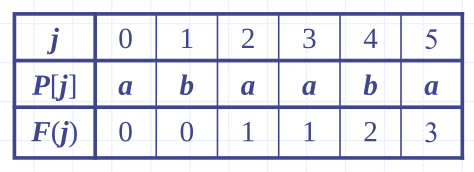
\includegraphics[width=.9\linewidth]{img/kmp_failure_function.png}
\caption{\label{fig:org0edff7b}Failure Function for KMP}
\end{figure}


\begin{algorithm}
  \caption{KMP Failure Function}
  \begin{algorithmic}[1]
    \Procedure{failureFunction}{$P$}
    \State $F[0] \leftarrow 0$
    \State $i \leftarrow 1$ \{ Location in pattern \}
    \State $j \leftarrow 0$ 
    \While{$i < m$}
    \If{$P[i] = P[j]$}
    \State $F[i] \leftarrow  j + 1$
    \State $i \leftarrow i + 1$
    \State $j \leftarrow j + 1$
    \ElsIf{$j > 0$}
    \State $j \leftarrow F[j-1]$
    \Else
    \State $F[i] \leftarrow 0$
    \State $i \leftarrow i + 1$
    \EndIf
    \EndWhile
    \textbf{return} -1 \{ no match \}
    \EndProcedure
  \end{algorithmic}
\end{algorithm}

\subparagraph{Tries} \
\label{sec:orgeab324a}

A \textbf{Trie} is a data structure (a tree \href{../../../roam/20210806224741-tree.org}{Tree}) to represent a set of strings.
Tries are used to perform fast pattern matching.


The Default-Trie / Standard-Trie has:
\begin{itemize}
\item each node except the root node has exactly one symbol
\item Every path from the root to a leaf is a word in the set
\end{itemize}


The Default-Trie stores every symbol in a node.
But sometimes a node has only one next node.
This symbol and the next node can be merged together in one node.


\begin{figure}[htbp]
\centering
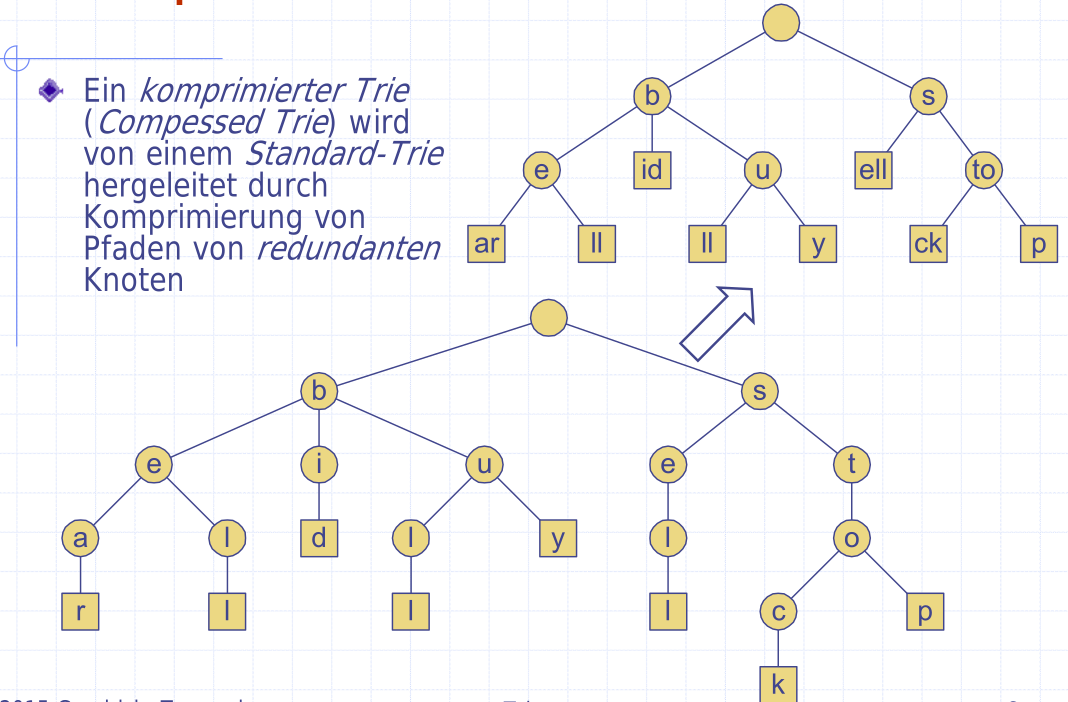
\includegraphics[width=.9\linewidth]{img/tries.png}
\caption{\label{fig:org7fcdff5}Example of Tries}
\end{figure}


The Suffix-Trie for a string is a compress trie (\href{../../../roam/20220201152933-tries.org}{Tries}) which stores all suffixes.

\begin{figure}[htbp]
\centering
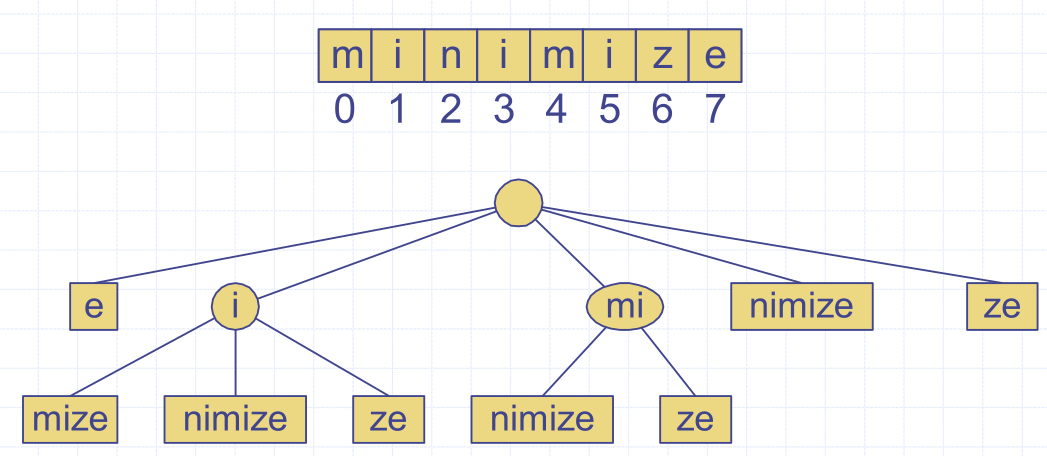
\includegraphics[width=.9\linewidth]{img/suffix_trie.png}
\caption{\label{fig:org3de1e5f}Suffix Trie}
\end{figure}

\subparagraph{DFS} \
\label{sec:org3f0cf13}

Depth-First search is a technique to traverse a \href{../../../roam/20220201163000-graph.org}{Graph}.
As the name says you go deep and then wide (see \ref{fig:org57a9bb3}).


\begin{figure}[htbp]
\centering
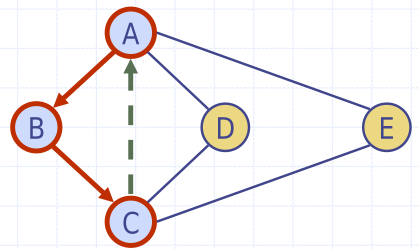
\includegraphics[width=.9\linewidth]{img/dfs.png}
\caption{\label{fig:org57a9bb3}DFS Example}
\end{figure}



\begin{algorithm}
  \caption{DFS Algorithm}
  \begin{algorithmic}[1]
    \Procedure{DFS}{$G$}
    \ForAll{$u \in G.vertices()$}
    \State $setLabel(u, UNEXPLORED)$
    \EndFor

    \ForAll{$e \in G.edges()$}
    \State $setLabel(e, UNEXPLORED)$
    \EndFor

    \ForAll{$v \in G.vertices()$}
    \If{$getLabel(v) = UNEXPLORED$}
    \State $DFS(G, v)$
    \EndIf
    \EndFor
    \EndProcedure
  \end{algorithmic}
  \begin{algorithmic}[1]
    \Procedure{DFS}{$G, v$}
    \State $setLabel(v, VISITED);$
    \ForAll{$e \in G.incidentEdges(v)$}
    \If{$getLabel(e) = UNEXPLORED$}
    \State $w \leftarrow opposite(v,e)$
    \If{$getLabel(w) = UNEXPLORED$}
    \State $setLabel(e, DISCOVERED)$
    \State $DFS(G, w)$
    \Else
    \State $setLabel(e, BACK)$
    \EndIf
    \EndIf
    \EndFor
    \EndProcedure
  \end{algorithmic}
\end{algorithm}

\subparagraph{DFS for finding path} \
\label{sec:org7f2a2aa}

\href{../../../roam/20220202095038-dfs.org}{DFS} can be used to find a path between two vertices in a \href{../../../roam/20220201163000-graph.org}{Graph}.
Every time you discovered a new edge, the edge is added to a stack.
If you come back from this edge (return from the recursion) you remove it from the stack.
If you finally found the searched vertex the path to this is stored in the stack.




\begin{algorithm}
  \caption{Find path with DFS}
  \begin{algorithmic}[1]
    \Procedure{pathDFS}{$G, v, z$}
    \State $setLabel(v, VISITED)$
    \State $S.push(v)$ \{ Stores the path \}
    \If{$v = z$}
    \State \textbf{finish: result is} $S.elements()$
    \EndIf
    \ForAll{$e \in G.incidentEdges(v)$}
    \If{$getLabel(e) = UNEXPLORED$}
    \State $w \leftarrow opposite(v, e)$
    \If{$getLabel(w) = UNEXPLORED$}
    \State $setLabel(e, DISCOVERY)$
    \State $S.push(e)$
    \State $pathDFS(G, w, z)$
    \State $S.pop()$
    \Else
    \State $setLabel(e, BACK$
    \EndIf
    \EndIf
    \EndFor
    \State $S.pop()$
    \EndProcedure
  \end{algorithmic}
\end{algorithm}

\subparagraph{DFS For finding cycleso} \
\label{sec:org6da6181}

\href{../../../roam/20220202095038-dfs.org}{DFS} can be used to find cycles in a \href{../../../roam/20220201163000-graph.org}{Graph}.
Using a stack you store the path from the start to the end vertex.
DFS has found a cycle as soon as you would mark a edge with \textbf{BACK}.


\begin{algorithm}
  \caption{Find Cycles with DFS}
  \begin{algorithmic}
    \Procedure{$cyclesDFS$}{$G, v$}
    \State $setLabel(v, VISITED)$
    \State $S.push(v)$
    \ForAll{$e \in G.incidentEdges(v)$}
    \If{$getLabel(e) = UNEXPLORED$}
    \State $w \leftarrow opposite(v, e)$
    \State $S.push(e)$
    \If{$getLabel(w) = UNEXPLORED$}
    \State $setLabel(e, DISCOVERY)$
    \State $cycleDFS(G, w)$
    \State $S.pop()$
    \Else
    \State $T \leftarrow new empty stack$
    \Repeat
    \State $o \leftarrow S.pop()$
    \State $T.push(0)$
    \Until{$o = w$}
    \State \textbf{finish: result in} $T.elements()$
    \EndIf
    \EndIf
    \EndFor
    \State $S.pop()$
    \EndProcedure
  \end{algorithmic}
\end{algorithm}

\subparagraph{BFS} \
\label{sec:orgdbdc341}

Breath-First Search is a technique to traverse a graph.
BFS visits one level after another.
The start vertex is marked as visited.
Then all adjacent vertexes are visited.
BFS uses a \href{../../../roam/20210806221243-queue.org}{Queue} to store which vertex should be visited next.


\begin{figure}[htbp]
\centering
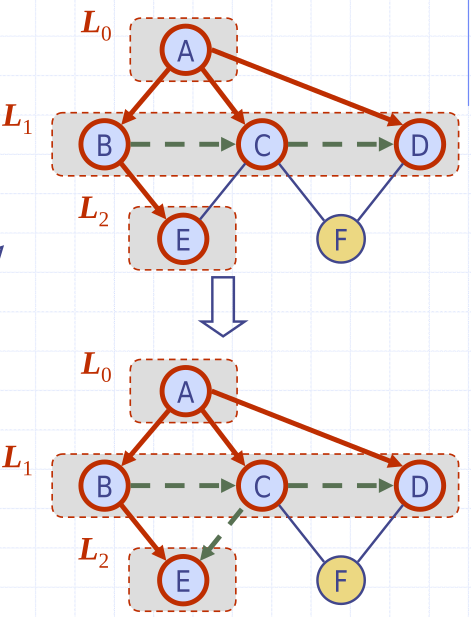
\includegraphics[width=.9\linewidth]{img/bfs_example.png}
\caption{\label{fig:orgb54a45b}BFS Example}
\end{figure}


\begin{algorithm}
  \caption{BFS Algorithm}
  \begin{algorithmic}
    \Procedure{$BFS$}{$G$}
    \ForAll{$u \in G.vertices()$}
    \State $setLabel(u, UNEXPLORED)$
    \EndFor

    \ForAll{$e \in G.edges()$}
    \State $setLabel(e, UNEXPLORED)$
    \EndFor

    \ForAll{$v \in G.evertices()$}
    \If{$getLabel(v) = UNEXPLORED$}
    \State $DFS(G, v)$
    \EndIf
    \EndFor
    \EndProcedure
  \end{algorithmic}
  \begin{algorithmic}
    \Procedure{$BFS$}{$G, s$}
    \State $L_0 \leftarrow new empty sequence$
    \State $L_0.insertLast(s)$
    \State $setLabel(s, VISITED)$
    \State $i \leftarrow 0$
    \While{$\neg L_i.isEmpty()$}
    \State $L_{i+1} \letarrow new empty sequence$
    \ForAll{$v \in L_i.elements()$}
    \ForAll{$e \in G.incidentEdges(v)$}
    \If{$getLabel(e) = UNEXPLORED$}
    \State $w \leftarrow opposite(v,e)$
    \If{$getLabel(w) = UNEXPLORED$}
    \State $setLabel(e, DISCOVERY)$
    \State $setLabel(w, VISITED)$
    \State $L_{i+1}.insertLast(w)$
    \Else
    \State $setLabel(e, CROSS)$
    \EndIf
    \EndIf
    \EndFor
    \EndFor
    \EndWhile
    \State $i \leftarrow i + 1$
    \EndProcedure
  \end{algorithmic}
\end{algorithm}

\subparagraph{DFS vs. BFS} \
\label{sec:org43cc70b}

A comparision of \href{../../../roam/20220202095038-dfs.org}{DFS} and \href{../../../roam/20220202102510-bfs.org}{BFS}.


\begin{figure}[htbp]
\centering
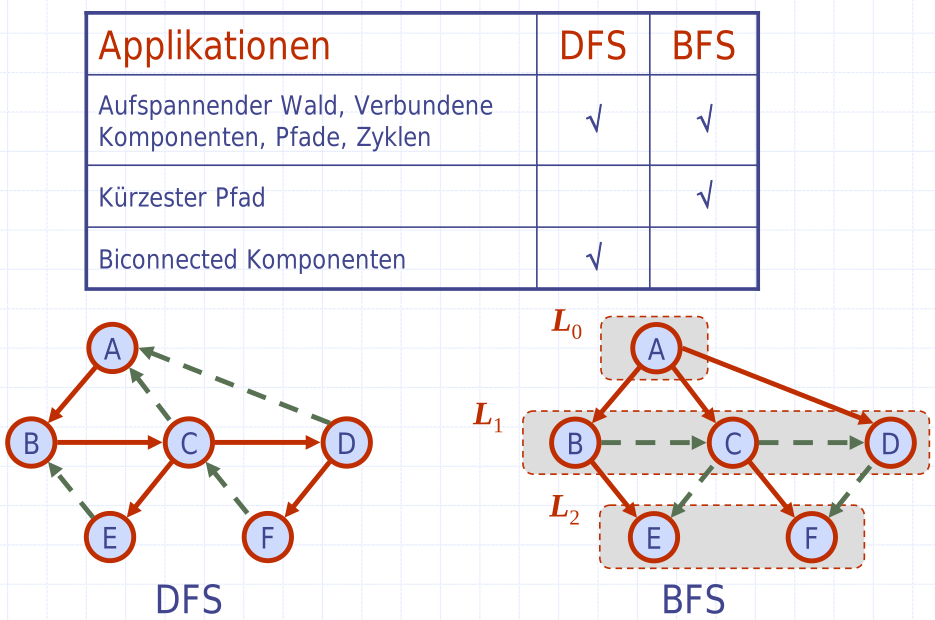
\includegraphics[width=.9\linewidth]{img/dfs_vs_bfs.png}
\caption{\label{fig:org649a30d}DFS vs. BFS}
\end{figure}

\subparagraph{Floyd-Warshall} \
\label{sec:org2365c76}

The Floyd-Warshall algorithm is used to calculate the Transitory closure of a \href{../../../roam/20220201163000-graph.org}{Graph} \(G\).


\begin{algorithm}
  \caption{Floyd-Warshall's Algorithm}
  \begin{algorithmic}
    \Procedure{$FloydWarshall$}{$G$}
    \State $i \gets 1$
    \ForAll{$v \in G.vertices()$}
    \State $denote v as v_i$
    \State $i \gets i + 1$
    \EndFor
    \State $G_0 \gets G$
    \For{$k \gets 1$ \textbf{to} $n$}
    \State $G_k \gets G_{k-1}$
    \For{$i \gets 1 \textbf{to} n (i \ne k)$}
    \For{$j \gets 1 \textbf{to} n (j \ne i,k)$}
    \If{$G_{k-1}.areAdjacent(v_i,v_k) \land G_{k-1}.areAdjacent(v_i, v_j)$}
    \If{$\neg G_k.areAdjacent(v_i, v_j)$}
    \State $G_k.insertDirectedEdge(v_i, v_j, k)$
    \EndIf
    \EndIf
    \EndFor
    \EndFor
    \EndFor
    \State \textbf{return} G_n
    \EndProcedure
  \end{algorithmic}
\end{algorithm}



From \(v_5\) to \(v_4\) exists a directed path over \(v_1\).
There for are \(j = 4, i = 5, k = 1\).


\begin{figure}[htbp]
\centering
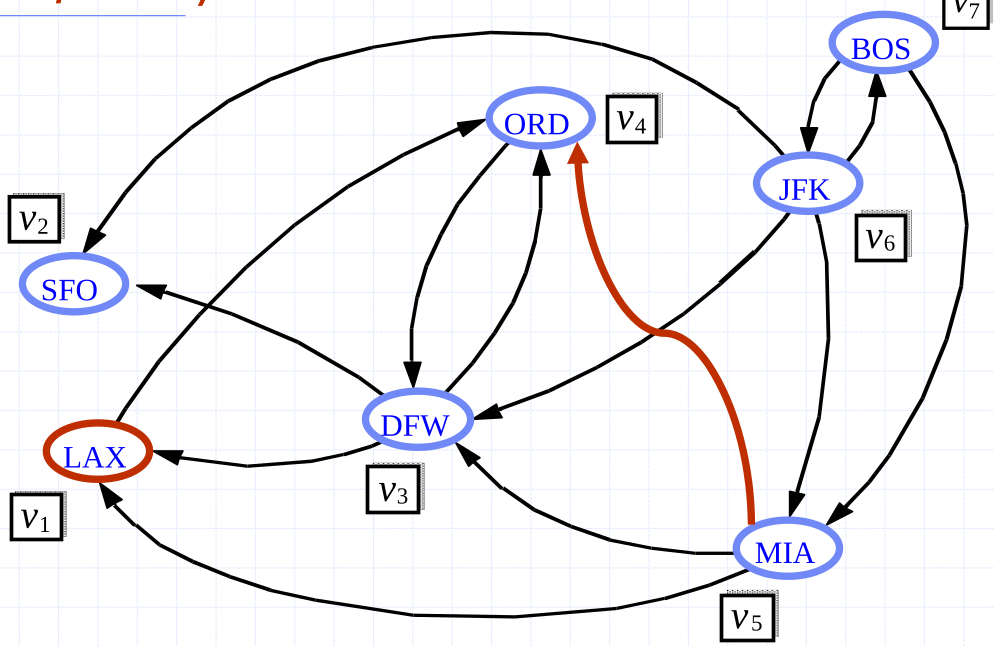
\includegraphics[width=.9\linewidth]{img/floyd_warshall.png}
\caption{\label{fig:org45157a4}Floyd-Warshall Example}
\end{figure}

\subparagraph{Topological Sorto} \
\label{sec:orgfc97db0}

Topological Sort is used to sort / enumerate vertices so that for an edge (\(u\), \(v\)) \(u < v\) true is.


\begin{figure}[htbp]
\centering
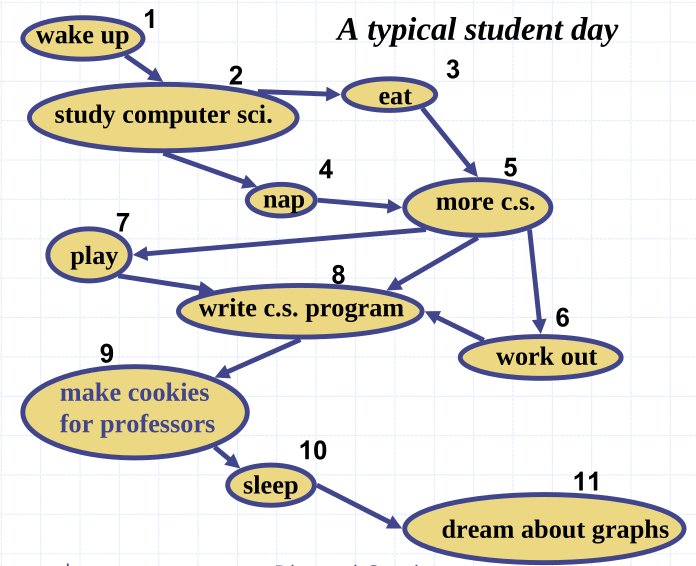
\includegraphics[width=.9\linewidth]{img/topological_sort_example.png}
\caption{\label{fig:orgb15c077}Topological Sort Example}
\end{figure}


Topological Sort is just a \href{../../../roam/20220202095038-dfs.org}{DFS} where you label the vertices.


\begin{algorithm}
  \caption{Topological Sort using DFS}
  \begin{algorithmic}[1]
    \Procedure{topologicalDFS}{$G$}
    \ForAll{$u \in G.vertices()$}
    \State $setLabel(u, UNEXPLORED)$
    \EndFor

    \ForAll{$e \in G.edges()$}
    \State $setLabel(e, UNEXPLORED)$
    \EndFor

    \ForAll{$v \in G.vertices()$}
    \If{$getLabel(v) = UNEXPLORED$}
    \State $topologicalDFS(G, v)$
    \EndIf
    \EndFor
    \EndProcedure
  \end{algorithmic}
  \begin{algorithmic}[1]
    \Procedure{topologicalDFS}{$G, v$}
    \State $setLabel(v, VISITED);$
    \ForAll{$e \in G.incidentEdges(v)$}
    \If{$getLabel(e) = UNEXPLORED$}
    \State $w \gets opposite(v,e)$
    \If{$getLabel(w) = UNEXPLORED$}
    \State $setLabel(e, DISCOVERED)$
    \State $topologicalDFS(G, w)$
    \Else
    \State $setLabel(e, n)$
    \EndIf
    \EndIf
    \EndFor
    \State $n \gets n - 1$
    \EndProcedure
  \end{algorithmic}
\end{algorithm}

\subparagraph{Dijkstra} \
\label{sec:orgb493fbf}

The Dijkstra Algorithm is used to calculate the distance to all vertices from a start vertex \(s\) in a \href{../../../roam/20220201163000-graph.org}{Graph}.
Dijkstra has a few requirements:
\begin{itemize}
\item The graph is connected
\item the edges are undirected
\item the edge weight is not negative
\end{itemize}


You build a cloud of vertices.
Beginning with the start vertex \(s\) you add one vertex after one to the cloud.
With each vertex \(v\) we store a property which holds the distance from \(s\) to \(v\).
After each iteration we add the vertex with the lowest distance and update the distance of all adjacent vectors.


\begin{figure}[htbp]
\centering
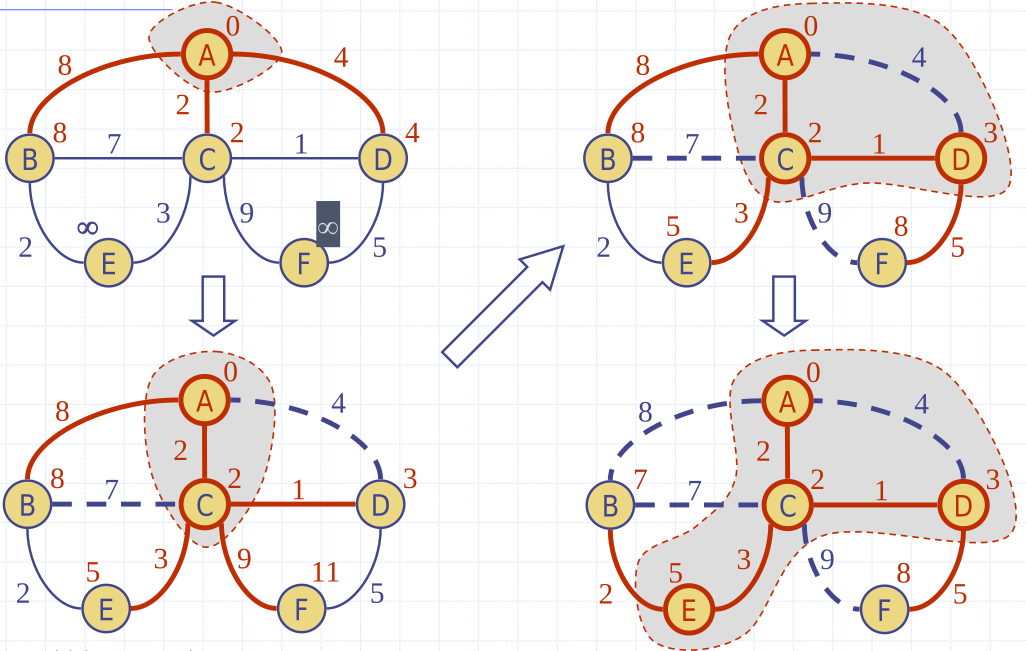
\includegraphics[width=.9\linewidth]{img/dijkstra_algorithm_example.png}
\caption{\label{fig:orgb13d651}Dijkstra Algorithm Example}
\end{figure}


\begin{algorithm}
  \caption{Dijkstra Algorithm}
  \begin{algorithmic}
    \Procedure{$DikstraDistance$}{$G, s$}
    \State $Q \gets$ new heap-based adaptable PQ
    \State \{ Initialization \}
    \ForAll{$v \in G.vertices()$}
    \If{$v = s$}
    \State $setDistance(v, 0)$
    \Else
    \State $setDistance(v, \infty)$
    \EndIf
    \EndFor

    \While{$\neg Q.isEmpty()$}
    \State $u \gets Q.removeMin().getValue()$
    \ForAll{$e \in G.incidentEdges(u)$}
    \State \{ relax edge e\}
    \State $z \gets G.opposite(u, e)$
    \State $r \gets getDistance(u) + weight(e)$
    \If{$r < getDistance(z)$}
    \State $setDistance(z,r)$
    \State $Q.replaceKey(getLocator(z), r)$
    \EndIf
    \EndFor
    \EndWhile
    \EndProcedure
  \end{algorithmic}
\end{algorithm}

\subparagraph{Bellman-Ford} \
\label{sec:orgab7b547}

The Bellman-Ford algorithm is use to caculate the distance from a vertex to every other vertex in a \href{../../../roam/20220201163000-graph.org}{Graph}.
But other then the \href{../../../roam/20220202132913-dijkstra_algorithm.org}{Dijkstra Algorithm} the Bellman-Ford algorithm can also work with negative edge weights.
Requirements:
\begin{itemize}
\item directed edges
\item no negative weighted cycles
\end{itemize}


\begin{algorithm}
  \caption{Bellman-Ford Algorithm}
  \begin{algorithmic}
    \Procedure{$BellmanFord$}{$G,s$}
    \ForAll{$v \in G.vertices()$}
    \If{$v = s$}
    \State $setDistance(v, 0)$
    \Else
    \State $setDistance(v, \infty)$
    \EndIf
    \EndFor

    \State $n \gets G.numVertices()$

    \For{$i \gets 1$ \textbf{to} $n-1$}
    \ForAll{$e \in G.edges()$}
    \State $u \gets G.origin(e)$
    \State $z \gets G.opposite(u,e)$
    \State $r \gets getDistance(u) + weight(e)$
    \If{$r < getDistance(z)$}
    \State $setDistance(z,r)$
    \EndIf
    \EndFor
    \EndFor
    \EndProcedure
  \end{algorithmic}
\end{algorithm}


\begin{figure}[htbp]
\centering
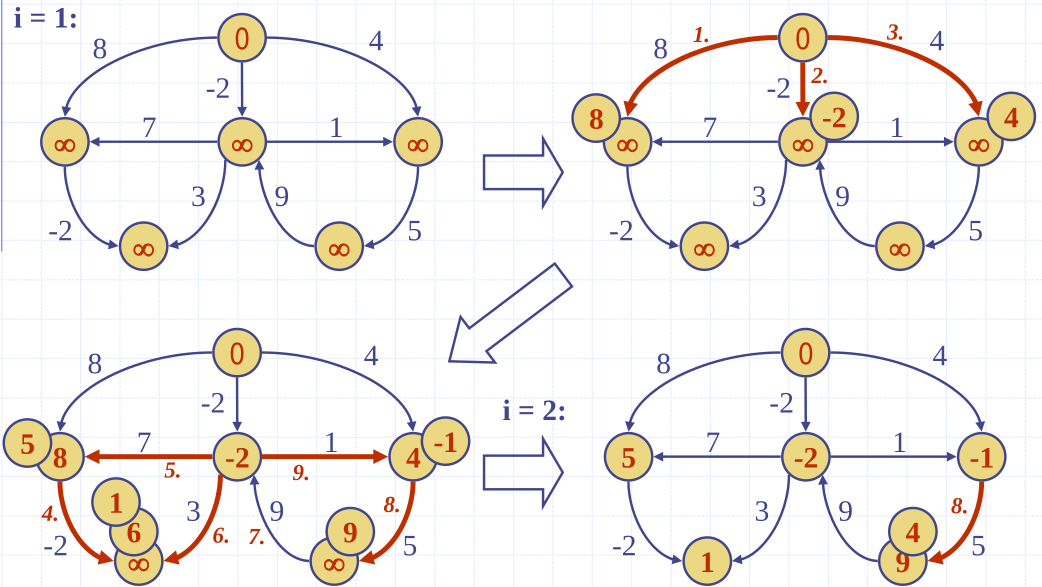
\includegraphics[width=.9\linewidth]{img/bellman_ford_example.png}
\caption{\label{fig:orgc468214}Bellman-Ford Example}
\end{figure}
\end{document}